\documentclass[11pt]{article}
\usepackage[margin=1in]{geometry}
\usepackage{url}

\def\R{\textsf{R}}
\def\Python{\textsf{Python}}
\def\Java{\textsf{Java}}
\def\RSNL{{\normalfont\fontseries{b}\selectfont RSNL}}
\def\tm{{\normalfont\fontseries{b}\selectfont tm}}
\def\xml{{\normalfont\fontseries{b}\selectfont xml}}
\def\stats{{\normalfont\fontseries{b}\selectfont stats}}

\let\code=\texttt
\let\rclass=\texttt

%% \VignetteIndexEntry{An Introduction to RSNL}

\usepackage{Sweave}
\begin{document}

\title{An Introduction to \RSNL}

\author{Anthony Fader, Gary King, Daniel Pemstein, and Kevin Quinn}

\maketitle

\section{Introduction}




\RSNL\ (\R\ Statistics with Natural Language) provides \R\ programmers
with access to an aRSeNaL of natural language processing (NLP) tools
they can use without leaving the \R\ environment.  \RSNL\ relies on S4
classes and generic functions to present programmers with a simple,
uniform, and extensible interface to natural language processing in
\R.  Specifically, it provides a suite of methods for common natural
language tasks (e.g. tokenization, stemming, part-of-speech tagging,
and topic modeling) and a collection of extensible S4 objects (e.g.
tokenizers, stemmers, taggers, and topic model objects) to use when
carrying out these operations.  Furthermore, \RSNL's toolset allows
the user to keep track of relationships between chunks of text---and
decompositions and summaries of those bits of text---throughout the
analysis process, using an \emph{object-view} model to provide
multiple, concurrent, representations of an underlying collection of
texts.  This \emph{object-view} approach facilitates exploratory data
analysis while simultaneously providing a powerful sub-structure upon
which to build high-level NLP analysis and visualization software.
Finally, while most publicly available NLP toolkits are designed to
meet the needs of natural language research, \RSNL\ is intended to
facilitate NLP-based analyses by applied researchers, particularly
those in the social and behavioral sciences, and is tuned to their
problems and their datasets.

This document provides a short, example-based, introduction to \RSNL\
that demonstrates how to prepare a text collection to
interact with \RSNL's toolset, how to pre-process the text using a
combination of \tm-based and \RSNL-provided tools, how to extend and
adapt these tools, and how to apply NLP tools to the text collection
to produce multiple \emph{views} of a text collection, or corpus.  As
development on \RSNL\ progresses, this document will also demonstrate
how to use \RSNL\ to better keep track of corpus structure and
meta-data, and explain the range of clustering and classification
methods, visualization tools, discourse modeling and testing
techniques, and topic modeling methods included in the \RSNL\ toolkit.

\section{Preparing a Dataset for Analysis}
\label{sec:prep}

\RSNL\ builds upon the text-processing middle-ware layer provided by
the \tm\ package to provide a multitude of text processing and
modeling tools.  \RSNL\ relies on \tm\cite{tm} to handle text
input-output, data management and storage.  \tm~provides S4
types---the \rclass{TextDocument} and \rclass{Corpus} classes---that
allow users to represent, examine, and manipulate individual chunks of
text (typically individual documents) and large corpora of related
documents.  Additionally, these basic data types sport fields for
maintaining detailed metadata about the underlying text.  Furthermore,
\tm~includes a wide array of I/O tools, including readers and writers
for various document formats, back-end database support, and functions
that allow users to apply transformations and filters to an individual
document or corpus with relative ease.  Finally, \tm~provides a simple
object, the \rclass{DocumentTermMatrix}, for representing corpora in terms
of document-level word frequencies.

\RSNL\ works intimately with \tm\ to prepare a text collection for
higher level analysis; \RSNL\ users will typically adopt the following
work-flow when preparing a set of documents for analysis:
\begin{enumerate} \item The user will use \tm's text I/O tools to read
a collection of documents into \R\ and create a \rclass{Corpus}
object.  \item The user will construct an \RSNL\
\rclass{RSNLCorpus} object from the newly minted \rclass{Corpus} to best
take advantage of \RSNL's collection of tools.  \item The user will
transform and filter the data as necessary to prepare it for
higher-level analysis; during this step, one will make use of \tm's
mapping and filtering functions to perform tasks that destructively
modify the text collection, while relying on \RSNL's collection of
tokenizers, stemmers, transforms, and filters to create a variety of
non-destructive \emph{views} of the underlying dataset.
\end{enumerate} The rest of this section explains this process in
detail.

\subsection{Working with Corpus Objects}

\begin{figure}
\begin{center}
\begin{verbatim}
<?xml version="1.0"?>
<DEBATE-SPEECH>
  <!-- 1. Bill-specific meta-data -->
  <BILL>
    <TITLE> Packaging and packaging waste</TITLE>
    <CODE>A6-0027/2004</CODE>
    <DATE>2004-11-17</DATE>
    <ITEM>5</ITEM>
    <RAPPORTEUR>CORBEY</RAPPORTEUR>
    <ISSUEAREA>3</ISSUEAREA>
    <PASSED>1</PASSED>
    <RCV>0</RCV>
  </BILL>

  <!-- 2. Speaker-specific meta-data -->
  <SPEAKER>
    <NAME>President</NAME>
    <COUNTRY></COUNTRY>
    <GROUP></GROUP>
    <STATUS>
      <ISPRESIDENT>1</ISPRESIDENT>
      <ISCOUNCIL>0</ISCOUNCIL>
      <ISCOMMISSION>0</ISCOMMISSION>
      <ISOTHERBUREAUCRAT>0</ISOTHERBUREAUCRAT>
      <ISRAPPORTEUR>0</ISRAPPORTEUR>
      <ISCOMMITTEEREP>0</ISCOMMITTEEREP>
      <ISAUTHOR>0</ISAUTHOR>
      <ISONBEHALFOFGROUP>0</ISONBEHALFOFGROUP>
    </STATUS>
  </SPEAKER>

  <!-- 3. Speaker ordering -->
  <SPEAKER-NUMBER>1</SPEAKER-NUMBER>

  <!-- 4. The text -->
  <TEXT>
    The next item is the report ( A6-0027/2004 ) by Mrs Corbey
    on the draft European Parliament and Council Directive amending
    Directive 94/62/EC on packaging and packaging waste.
  </TEXT>
</DEBATE-SPEECH>
\end{verbatim}
\caption{An example EP speech in XML format.}
\label{fig:xml}
\end{center}
\end{figure}

Throughout this document we will work with an example dataset
containing a selection of 475 short speeches given by legislators and
bureaucrats during debates on legislation in the European Parliament
(EP).  The speeches are a (non-random) sample from a larger dataset of
EP debates \cite{rcv}.  The dataset has a
hierarchical structure and each speaker delivered her speech as part
of a debate dedicated to a particular piece of legislation.
Specifically, each speech fits into one of the first 29 debates on
Codecision\footnote{The European Parliament considers legislation
under a variety of legislative procedures.  Codecision is generally
considered the most important of these procedures although the
particulars of EP protocol are of little consequence to the current
example.} legislation conducted by the Parliament in its 6th (current)
term.  These data ship with \RSNL\ as a series of XML documents which
contain both the raw text of the speeches and a variety of meta-data.

Figure~\ref{fig:xml} displays one of the XML documents in the example
dataset.  Each file is composed of four main sections.   The first
section contains the bill's title, unique EP code, date of debate,
position on the day's debate schedule, the last name of the member of
the EP (MEP) responsible for reporting on the bill, a number
indicating one of eight policy issue areas assigned to the bill by EU
bureaucrats, a dummy variable indicating whether or not the reading of
the bill survived a vote on the legislation as a whole, and a binary
indicator of whether or not that final vote was conducted by public
roll call.  The second section provides speaker-specific information
including the speaker's name (or title, if the speaker is acting in a
purely institutional role), the country and parliamentary party group
the speaker represents (if applicable), and a series of dummy
variables describing the speaker's institutional role vis-a-vis the
given piece of legislation.  Finally, the third section of the xml
file contains a single indicator identifying the chronological
position of the speech in the debate while the fourth section sports
the raw text of the speech itself.

\tm\ represents collections of documents using the
\rclass{Corpus} data structure which can read text from a disk or
other \rclass{Source} using either a pre-defined or custom
\code{reader} function.  Therefore, our first step in any analysis of
the EP speeches will be to construct a \tm-style reader and use it
to build a \rclass{Corpus} object from our XML files on disk.
\begin{Schunk}
\begin{Sinput}
> library(RSNL)
> library(XML)
> # Define a custom reader, see tm docs for details
> readSpeeches <- FunctionGenerator(function(...) {
+   function (elem, load, language, id) {
+     # 1. Get the xml nodes organized
+     tree <- xmlTreeParse(elem$content, asText = TRUE)
+     root <- xmlRoot(tree)
+     bill <- root[["BILL"]]          # bill-specific data
+     speaker <- root[["SPEAKER"]]    # speaker-specific data
+     status <- speaker[["STATUS"]]   # institutional context dummies
+     
+     # 2. Create the default meta-data fields
+     title <- paste(xmlValue(bill[["TITLE"]]), "-",
+                    xmlValue(speaker[["NAME"]]), sep="")
+ 
+     dateTimeStamp <- as.POSIXct(xmlValue(bill[["DATE"]]), tz="CET")
+ 
+     id <- paste(xmlValue(bill[["CODE"]]),
+                 xmlValue(root[["SPEAKER-NUMBER"]]), sep=".")
+ 
+     content <- xmlValue(root[["TEXT"]])
+ 
+     # 3. Construct the document
+     doc<-new("PlainTextDocument", .Data = content,
+         Author = "European Parliament",
+         DateTimeStamp = dateTimeStamp, 
+         Origin = "http://www.europarl.europa.eu", Heading = title,
+         Language = language, ID= id)
+ 
+     # 4. Add some custom metadata
+     meta(doc, "SPEAKER-NUMBER") <- xmlValue(root[["SPEAKER-NUMBER"]])
+ 
+     for (name in c("CODE", "ISSUEAREA", "PASSED", "RCV"))
+       meta(doc, name) <- xmlValue(bill[[name]])
+ 
+     for (name in c("COUNTRY", "GROUP"))
+       meta(doc, name) <- xmlValue(speaker[[name]])
+ 
+     for (name in c("ISPRESIDENT", "ISCOUNCIL", "ISCOMMISSION",
+                    "ISOTHERBUREAUCRAT", "ISRAPPORTEUR", "ISCOMMITTEEREP",
+                    "ISAUTHOR", "ISONBEHALFOFGROUP"))
+       meta(doc, name) <- xmlValue(status[[name]])
+ 
+     doc
+   }
+ })
\end{Sinput}
\end{Schunk}
The \code{readSpeeches()} function in the code snipped above is a
\rclass{FunctionGenerator}; that is, rather than returning a standard
object when called, \code{readSpeeches()} returns a function.
Specifically, each invocation of \code{readSpeeches()} returns a
function that takes information about a single element (that is,
document) read from a source---the element itself, loading info which
we ignore here, the document language, and a document id---and returns
a \rclass{PlainTextDocument} suitable for inclusion in a
\rclass{Corpus}.  In this case, we use the \xml\ package\cite{xml} to
parse each EP speech in XML format and populate the fields and
metadata slots of each resulting
\rclass{PlainTextDocument}.\footnote{The \code{FunctionGenerator()}
function call in the above code acts only to set the type (i.e.
\rclass{FunctionGenerator}) of the resulting function-generating
object.  Remember that, in \R, functions are objects and can carry
type information.  For type safety, \tm's \rclass{Corpus}
constructor expects all readers to be \rclass{FunctionGenerator}
objects.  In fact, the code \code{FunctionGenerator(function (...) {
function () })} is equivalent to \code{new("FunctionGenerator", .Data
= function (...) { function () })}.}  The first chunk of the function
returned by \code{readSpeeches()}
sets up convenience handles to the XML nodes representing the
bill-specific meta-data, speaker-specific information, and the dummy
variables related to the institutional responsibilities of the
speaker.  Section two extracts a variety of specific fields from the
XML document and uses them to fill in the \rclass{PlainTextDocument}'s
default fields; specifically, it generates a title by concatenating
the bill's title to the speaker's name, converts the date of the
debate into a timestamp, generates a document id by concatenating the
bill code to the speaker's chronological position in the debate, and
extracts the content of the speech itself.  Next, section three
constructs the \rclass{PlainTextDocument} object using the variables
extracted in the first two portions of the function.  Finally, the
fourth and last chunk of code appends a variety of meta-data to the
\rclass{PlainTextDocument}, using \tm's \code{meta()} method.  With
this reader in hand, we can create a connection to the EP dataset
included with \RSNL\ and pass the connection and reader to the
\rclass{Corpus} constructor provided by \tm:
\begin{Schunk}
\begin{Sinput}
> debates.source <- system.file("samples/en/ep-debates", package="RSNL")
> tm.debates <- Corpus(DirSource(debates.source), readerControl =
+                      list(reader = readSpeeches, language="EN"))
\end{Sinput}
\end{Schunk}

\subsubsection{Corpora and Passing Semantics}

Currently, \rclass{Corpus} objects may store their internal data
either directly in memory, or in a simple database format.  When using
in-memory storage, \rclass{Corpus} objects use \R's standard
\emph{pass-by-value} semantics.  This means that whenever a \rclass{Corpus}
is passed to a function or method the interpreter makes a copy of the
object and any changes to the object made within the function are not
reflected in the original object.  Furthermore, if we were to make a
simple copy of \code{tm.debates}
\begin{Schunk}
\begin{Sinput}
> tm.debates.copy <- tm.debates
\end{Sinput}
\end{Schunk}
\code{tm.debates.copy} and \code{tm.debates} would represent distinct
collections of text and changes to one object would have no effect on
the other.  On the other hand, when a
\rclass{Corpus} stores its data on disk, it uses
\emph{pass-by-reference} semantics; in this case \rclass{Corpus}
objects are essentially handles to an underlying data store and
multiple copies of the handle all refer to the same set of data.
Under these circumstances modifications to \code{tm.debates.copy}
would be reflected in subsequent calls to \code{tm.debates}.

This variance in \rclass{Corpus} passing semantics is simply a matter
of practicality.  When a \rclass{Corpus} maintains its data in memory
it is constrained by \R's default behavior to make copies of the text
it represents whenever copied or passed to a function.  On the other
hand, a \rclass{Corpus} object only needs to copy its database handle
when storing its text on disk; under these circumstances the \tm\
developers are able to conserve processor cycles and disk space by
leaving the data in one place while allowing the user to manipulate
references to the underlying data in \R\ itself.  Yet, while logical,
these implementation-dependent differences in \rclass{Corpus} passing
semantics may risk some potential confusion for users and, in the case
of in-memory storage, inefficiency.

\subsubsection{\rclass{RSNLCorpus} and Reference Objects}

\RSNL\ provides a wrapper class for \rclass{Corpus} objects,
\rclass{RSNLCorpus}, that unifies corpus semantics.
\rclass{RSNLCorpus}
objects behave exactly like \rclass{Corpus} objects\footnote{At the
current stage of development this not quite true: we have not
implemented the \code{c()} method for \rclass{RSNLCorpus} objects, nor
have we tested their compatibility with \tm's lazy mapping
facilities.} except that they use \emph{pass-by-reference} semantics
regardless of their underlying storage model.  Furthermore, they
provide under-the-hood tools that facilitate the data-view model
employed by \RSNL\, which we describe in more detail below.  Thus, the
second step in any \RSNL\ analysis is to convert a corpus represented
by \tm's \rclass{Corpus} type into a \rclass{RSNLCorpus}.  Doing this is
exceedingly simple; one need only pass an existing \rclass{Corpus} to
the \rclass{RSNLCorpus} constructor:
\begin{Schunk}
\begin{Sinput}
> debates <- RSNLCorpus(tm.debates)
\end{Sinput}
\end{Schunk}
\rclass{RSNLCorpus} objects are an example of a non-standard type of S4
object used throughout \RSNL: \rclass{RObject} or reference objects.
These objects pass one or more of their internal slots by reference
when one makes a copy or passes the object to a function.  It is
possible to force the interpreter to make a pure copy of a
\rclass{RObject} using the \code{clone()} method:
\begin{Schunk}
\begin{Sinput}
> debates.copy <- clone(debates)              # 1
> debates.copy.ref <- debates.copy            # 2
> debates.copy[[1]] <- debates.copy[[2]]      # 3
> debates[[1]] == debates.copy[[1]]           # 4
\end{Sinput}
\begin{Soutput}
[1] FALSE
\end{Soutput}
\begin{Sinput}
> debates.copy.ref[[1]] == debates.copy[[1]]  # 5
\end{Sinput}
\begin{Soutput}
[1] TRUE
\end{Soutput}
\end{Schunk}
It is worth walking through the above example, step by step, to
make the distinction between a reference and a pure copy absolutely
clear.  In step one we take the \rclass{RSNLCorpus} \code{debates}, which
stores its text data in memory, and make a pure copy of it called
\code{debates.copy}.  At this point we have two full copies of the
corpus in memory.  In step two we make a reference to
\code{debates.copy} called \code{debates.copy.ref}.  This step does
not make an additional copy of the underlying corpus and
\code{debates.copy} and \code{debates.copy.ref} behave simply as two
different names for the same underlying dataset.  In step three we
take advantage of the subset operator for \rclass{RSNLCorpus} objects,
which allows us to access a single document within a corpus, to
overwrite the first document in \code{debates.copy} with the second
document in the same corpus.  Steps four and five demonstrate how this
modification is reflected in the three \rclass{RSNLCorpus} objects and
highlight the fact that \code{debates} and \code{debates.copy}
reference distinct underlying datasets while \code{debates.copy} and
\code{debates.copy.ref} reference a single, shared, corpus.

\subsection{Tokenization and View Construction}\label{sec:tokenview}

Natural language models typically rely on patterns of tokens within
the data.  Tokens are often individual words, but can, in principle,
represent the output of any procedure that splits a single piece of
text into individual chunks.  In this example, we'll take the
traditional approach to tokenization and attempt to represent, or
view, each document in the corpus as a series of individual words.  To
do so, we need to clean up the text a bit---transform the text to all
lowercase, remove punctuation, numbers (which we'll represent using a
single token), and common words---and do the actual tokenization.  In
this example, we'll also employ a common technique known as stemming,
which reduces similar words with different suffixes (e.g. run, runner,
running) to common roots (e.g. run).  Finally, we'll ignore especially
short words when modeling the text.

The above-mentioned procedures all do varying degrees of violence to
the original text.  In English, converting the documents to lowercase
will have little impact on our ability to refer back to and understand
the content of the original documents while performing an exploratory
analysis, but other operations, such as transforming or eliminating
certain symbols or strings, tokenizing, and stemming, can render the
original text unreadable.  \RSNL\ takes advantage of an
\emph{object-view} model to help overcome this issue.  When performing
basic text-cleaning operations, such as converting the text to lower
case, the analyst will often wish to employ \tm's various filtering
and mapping tools to modify the \rclass{Corpus} itself.  But when
performing more destructive operations the analyst can benefit by
creating \emph{views} of the underlying \rclass{Corpus}, or its
constituent documents, that encapsulate both a reference to the
original text and a policy for transforming the text in some way.  Of
course, there is a trade-off here:  iteratively modifying the text in
place requires less storage space than the \emph{object-view} approach
and may be necessary with large datasets; on the other hand, the
\emph{object-view} model makes it far easier for the analyst to refer
back to the underlying data and work with multiple representations
(views) of the data at once, and will generally use fewer resources
than maintaining a copy of the corpus for each desired representation
of the data.

\subsubsection{Working with Tokenized Views}

We'll start by constructing a simple tokenized view of the corpus.
\RSNL\ provides a method, \code{tokenize()} that can generate tokens
from a variety of data types.  At the most basic level, given a
\code{character} object (or child type such as \tm's
\rclass{PlainTextDocument}), \code{tokenize()} will return a vector of
tokens:
\begin{Schunk}
\begin{Sinput}
> tokenize(debates[[1]])
\end{Sinput}
\begin{Soutput}
 [1] "The"          "next"         "item"        
 [4] "is"           "the"          "report"      
 [7] "-LRB-"        "A6-0027"      "\\/"         
[10] "2004"         "-RRB-"        "by"          
[13] "Mrs"          "Corbey"       "on"          
[16] "the"          "draft"        "European"    
[19] "Parliament"   "and"          "Council"     
[22] "Directive"    "amending"     "Directive"   
[25] "94\\/62\\/EC" "on"           "packaging"   
[28] "and"          "packaging"    "waste"       
[31] "."           
\end{Soutput}
\end{Schunk}
On the other hand, given a \rclass{RSNLCorpus}, \code{tokenize()} will
generate a view of that corpus:
\begin{Schunk}
\begin{Sinput}
> (debates.tok <- tokenize(debates))
\end{Sinput}
\begin{Soutput}
A tokenized corpus view with 179959 total tokens and 9265 unique tokens
\end{Soutput}
\end{Schunk}
In some cases, one might wish to obtain a view of a single document
within a corpus.  In this case, a user may employ the \code{index}
argument to \code{tokenize()} to select an individual document from
within the corpus.\footnote{Note that a view of a document maintains a
policy for representing the document (in this case a tokenization
policy) while keeping track of what corpus the document comes from.
Thus, applying \code{tokenize} to a corpus and using the \code{index}
argument is quite distinct from applying tokenize directly to a
document within a corpus, which simply generates a vector of tokens.
We discuss views in greater detail below.} For example, this code
creates a view of the first document in \code{debates}:
\begin{Schunk}
\begin{Sinput}
> (debates.tok.1 <- tokenize(debates, index=1))
\end{Sinput}
\begin{Soutput}
A tokenized document view of A6-0027/2004.1 with 31 total tokens and 26 unique tokens
\end{Soutput}
\end{Schunk}
\code{debates.tok} and \code{debates.tok.1} are examples of
\rclass{View} objects; specifically, \code{debates.tok} is a
\rclass{TokenizedCorpusView} and \code{debates.tok.1} is a
\rclass{TokenizedDocumentView}, both of which are sub-types of the
\code{TokenizedView}, and more generically, \rclass{View} virtual
classes.  All \rclass{View} objects provide a representation of a
given \rclass{RSNLCorpus} object.  Each view maintains a \emph{reference}
to a \rclass{RSNLCorpus} and encapsulates a policy for representing that
corpus.  For example, a \rclass{TokenizedCorpusView} of \code{debates}
contains a reference to \code{debates} and information about the
\rclass{Tokenizer} object\footnote{We describe \rclass{Tokenizer}
objects in more detail below.} used to break the text in
\code{debates} into individual tokens.  Similarly, a
\rclass{TokenizedDocumentView} references a single document within a
\rclass{RSNLCorpus} while maintaining a policy for representing that
document as a sequence of tokens.\footnote{Note that views are only
defined in reference to \rclass{RSNLCorpus} objects.  Therefore, you can
not create a view to a document not contained in a corpus.}
Furthermore, \rclass{View}s use a lazy approach and perform no actual
computation until absolutely necessary.  This means that, when
you use \code{tokenize()} to create a view of a given corpus, the
method performs no actual tokenization, but rather constructs a
\rclass{View} that is committed to representing the corpus in a
particular (tokenized) way.  The tokenization only occurs when the
user invokes further methods on the \rclass{TokenizedView}, as we
discuss below.  

We can examine our \rclass{TokenizedView}s with a variety of
methods.  For example, given the two views we just constructed, we can
look at the tokens within the first document in the corpus in one of
two ways:
\begin{Schunk}
\begin{Sinput}
> tokens(debates.tok[[1]])
\end{Sinput}
\begin{Soutput}
 [1] "The"          "next"         "item"        
 [4] "is"           "the"          "report"      
 [7] "-LRB-"        "A6-0027"      "\\/"         
[10] "2004"         "-RRB-"        "by"          
[13] "Mrs"          "Corbey"       "on"          
[16] "the"          "draft"        "European"    
[19] "Parliament"   "and"          "Council"     
[22] "Directive"    "amending"     "Directive"   
[25] "94\\/62\\/EC" "on"           "packaging"   
[28] "and"          "packaging"    "waste"       
[31] "."           
\end{Soutput}
\begin{Sinput}
> tokens(debates.tok.1)
\end{Sinput}
\begin{Soutput}
 [1] "The"          "next"         "item"        
 [4] "is"           "the"          "report"      
 [7] "-LRB-"        "A6-0027"      "\\/"         
[10] "2004"         "-RRB-"        "by"          
[13] "Mrs"          "Corbey"       "on"          
[16] "the"          "draft"        "European"    
[19] "Parliament"   "and"          "Council"     
[22] "Directive"    "amending"     "Directive"   
[25] "94\\/62\\/EC" "on"           "packaging"   
[28] "and"          "packaging"    "waste"       
[31] "."           
\end{Soutput}
\end{Schunk}
Furthermore, we can easily see the most common words in the corpus
\begin{Schunk}
\begin{Sinput}
> sort(freqTable(debates.tok), dec=T)[1:20]
\end{Sinput}
\begin{Soutput}
  the     ,     .    of    to   and    in  that    is 
10727  9467  6253  5710  5489  4823  3261  3045  2832 
    a   for     I    on    be  this    we    it   are 
 2752  2383  1871  1665  1603  1573  1374  1195  1188 
  not  have 
 1157  1121 
\end{Soutput}
\end{Schunk}
or generate a list of unique tokens:
\begin{Schunk}
\begin{Sinput}
> u <- unique(debates.tok)
\end{Sinput}
\end{Schunk}
Each of these operations requires the view to invoke its policy---the
\rclass{Tokenizer} it encapsulates---on the \rclass{RSNLCorpus} it refers
to.  The first code snippet requires only that the view tokenize the
first document in the corpus, but the latter two examples require the
view to tokenize the entire corpus.  If you perform these actions in
order you will notice that the interpreter spends substantially more
time generating the frequency table than it does generating the unique
tokens.  This is because the view stores the results of previous
computations for later use and need not re-tokenize the corpus when
generating the list of unique terms.\footnote{One can adjust a view's
storage behavior using the \code{keepComputed()} and
\code{keepDocumentViews()} methods.}

By default, \code{tokenize()} uses a tokenizer that breaks up the text
according to Penn Treebank conventions, but the package provides a
number of pre-defined \rclass{Tokenizer} types and users are free to
extend this base class to define their own.  For example, to emulate
the tokenizing done within \tm's \code{termFreq()} function we might
define a custom \rclass{Tokenizer} like so:
\begin{Schunk}
\begin{Sinput}
> setClass("TmTokenizer", representation("Tokenizer", fun="function")) # 1
\end{Sinput}
\begin{Soutput}
[1] "TmTokenizer"
\end{Soutput}
\begin{Sinput}
> TmTokenizer <- function ()                                           # 2
+   new("TmTokenizer", fun = function (x)
+     unlist(strsplit(gsub("[^[:alnum:]]+", " ", x    ), " ", fixed = TRUE)))
> setMethod("tokenize", signature(object="character",                  # 3
+                                 tokenizer="TmTokenizer",
+                                 index="missing"),
+   function (object, tokenizer, index) tokenizer@fun(object))
\end{Sinput}
\begin{Soutput}
[1] "tokenize"
\end{Soutput}
\end{Schunk}
In the first step (1) we define a new S4 class, \rclass{TmTokenizer}, that
extends the base \rclass{Tokenizer} class and includes a slot for a
tokenizing function.  Next (2) we create a constructor function for
\rclass{TmTokenizer}s that takes no arguments and returns a
\rclass{TmTokenizer} object with a set tokenizing function that uses
\R's regular expression tools to remove all of the non-alpha-numeric
characters from a character string and converts the string into
tokens by splitting the string at spaces.  Finally, (3) we
implement a specialization of the \code{tokenize()} method for the
signature \code{signature(object="character", tokenizer="TmTokenizer",
index="missing")} so that, when one passes a \rclass{character} object
and a \rclass{TmTokenizer} to \code{tokenize()}, it takes the given string
and applies the set tokenizing function to that string, returning a
sequence of tokens.  In general, when implementing a new
\rclass{Tokenizer} called, say, \rclass{MyTokenizer}, one need only
implement the specialization of \code{tokenize()} for the signature
\code{signature(object="character", tokenizer="MyTokenizer",
index="missing")}; \RSNL\ provides the rest of the method
specializations necessary to make the \rclass{Tokenizer} work with
\rclass{RSNLCorpus} and \rclass{View} objects.

While our \rclass{TmTokenizer} relies on \R's regular expression
engine to identify tokens, \RSNL's \rclass{RegexTokenizer} type allows
users to define arbitrary regex-based tokenizers that match strings
using the---often substantially faster---\Java\ regular expression
engine.  For example, we might construct a very simple tokenizer that
splits strings solely on whitespace using the following
definition (the second argument tells the tokenizer to match the
spaces in between tokens, rather than tokens):\footnote{Note the
double-escaping of character classes.}
\begin{Schunk}
\begin{Sinput}
> space.breaker <- RegexTokenizer("\\s+", matchToken = FALSE)
\end{Sinput}
\end{Schunk}
Note that all three tokenizers we've used thus far generate slightly
different representations of the underlying text.  The
\code{tokenize()} method takes a \rclass{Tokenizer} as its second
argument.  Thus, the three calls below call \code{tokenize()} with the
default tokenizer, a \rclass{TmTokenizer}, and using our custom
\rclass{RegexTokenizer}, respectively:
\begin{Schunk}
\begin{Sinput}
> tokenize(debates[[1]])
\end{Sinput}
\begin{Soutput}
 [1] "The"          "next"         "item"        
 [4] "is"           "the"          "report"      
 [7] "-LRB-"        "A6-0027"      "\\/"         
[10] "2004"         "-RRB-"        "by"          
[13] "Mrs"          "Corbey"       "on"          
[16] "the"          "draft"        "European"    
[19] "Parliament"   "and"          "Council"     
[22] "Directive"    "amending"     "Directive"   
[25] "94\\/62\\/EC" "on"           "packaging"   
[28] "and"          "packaging"    "waste"       
[31] "."           
\end{Soutput}
\begin{Sinput}
> tokenize(debates[[1]], TmTokenizer())
\end{Sinput}
\begin{Soutput}
 [1] "The"        "next"       "item"      
 [4] "is"         "the"        "report"    
 [7] "A6"         "0027"       "2004"      
[10] "by"         "Mrs"        "Corbey"    
[13] "on"         "the"        "draft"     
[16] "European"   "Parliament" "and"       
[19] "Council"    "Directive"  "amending"  
[22] "Directive"  "94"         "62"        
[25] "EC"         "on"         "packaging" 
[28] "and"        "packaging"  "waste"     
\end{Soutput}
\begin{Sinput}
> tokenize(debates[[1]], tokenizer=space.breaker)
\end{Sinput}
\begin{Soutput}
 [1] "The"          "next"         "item"        
 [4] "is"           "the"          "report"      
 [7] "("            "A6-0027/2004" ")"           
[10] "by"           "Mrs"          "Corbey"      
[13] "on"           "the"          "draft"       
[16] "European"     "Parliament"   "and"         
[19] "Council"      "Directive"    "amending"    
[22] "Directive"    "94/62/EC"     "on"          
[25] "packaging"    "and"          "packaging"   
[28] "waste."      
\end{Soutput}
\end{Schunk}
In what follows, we'll use the \rclass{TokenizedCorpusView} named
\code{debates.tok} that we created with the default tokenizer.

\subsection{Filters and Transforms}

As we mentioned at the beginning of section~\ref{sec:tokenview},
we're going to need to transform our text in a number of ways to make
it amenable to analysis.  First of all, because it has little impact
on the readability of the text, we'll start out by using \tm's
\code{tmpMap()} function to convert our text to lower-case.
\begin{Schunk}
\begin{Sinput}
> debates.tok
\end{Sinput}
\begin{Soutput}
A tokenized corpus view with 179959 total tokens and 9265 unique tokens
\end{Soutput}
\begin{Sinput}
> tmMap(debates, tmTolower)
\end{Sinput}
\begin{Soutput}
A corpus with 475 text documents
\end{Soutput}
\begin{Sinput}
> debates.tok
\end{Sinput}
\begin{Soutput}
A tokenized corpus view with 179958 total tokens and 8535 unique tokens
\end{Soutput}
\end{Schunk}
This sequence of operations illustrates one nice perk of \RSNL's
\emph{object-view} model: auto-updating.  As we previously noted,
\rclass{View} objects maintain references to the objects that they
view.  One advantage of this approach is the ability to quickly
examine an original document in light of something one finds in a
view; another is that views can keep track of when anything changes in
the underlying data structure and update to reflect modifications.
This auto-updating ability saves users from the tedious task of
redefining views after making changes to a corpus, something that can
save many key-strokes---or executions of the \code{source()}
function---when one performs an exploratory analysis on a dataset.

\subsubsection{Token Transforms and Filters}

As demonstrated briefly above, one can use \tm's \code{tmMap()} method
to modify the text contained within a \rclass{RSNLCorpus} object.
Nonetheless, this approach modifies the corpus directly and, as we
previously argued, it may often be useful to work with numerous
modified representations of the text without rendering the corpus
unreadable.  Therefore, we'll use \RSNL's filtering and transformation
methods to take care of the more destructive tasks we need to perform
to get the dataset ready for analysis and generate filtered and transformed
\rclass{TokenizedCorpusView}s of the underlying corpus to get these
jobs done:
\begin{Schunk}
\begin{Sinput}
> debates.tok <- filterTokens(debates.tok)              #1
> debates.tok <- filterTokens(debates.tok,              #2
+   PunctTokenFilter())
> debates.tok <- filterTokens(debates.tok,              #3
+   FunctionalTokenFilter(function (x) nchar(x) > 3))
> debates.tok <- transformTokens(debates.tok,           #4
+   RegexTokenTransform("^[0-9]+$", "NUMBER"))
> debates.tok <- stem(debates.tok)                      #5
> debates.tok <- filterTokens(debates.tok,              #6
+   RegexTokenFilter("^[^a-zA-Z]+$", negate=TRUE))
> debates.tmp <- debates.tok  # Save for bigrams example   
> debates.tok <- filterTokens(debates.tok,              #7
+   TokenDocFreqFilter(debates.tok, .05, .95))
> debates.tok
\end{Sinput}
\begin{Soutput}
A tokenized corpus view with 41262 total tokens and 462 unique tokens
\end{Soutput}
\begin{Sinput}
> sort(freqTable(debates.tok), dec=T)[1:20]
\end{Sinput}
\begin{Soutput}
  european     propos    commiss    program 
       786        713        674        506 
    direct      amend     presid     report 
       497        463        434        359 
parliament     NUMBER   committe    support 
       355        348        313        306 
      time    protect      europ      peopl 
       273        267        257        255 
    energi     safeti      thank particular 
       254        252        252        249 
\end{Soutput}
\end{Schunk}
These operations take advantage of \RSNL's \code{filterTokens()},
\code{transformTokens()}, and \code{stem()} methods to (1) filter out
common English words,\footnote{The default behavior of
\code{filterTokens()} is to remove stop-words.  To see a list of
stopwords, type \code{stopwords("english")} at the \R\ prompt.} (2)
remove all-punctuation tokens, (3) filter tokens shorter than three
characters in length, (4) convert all-numeric tokens to the catch-all
token ``NUMBER'', (5) reduce the tokens to common roots, (6) remove
all remaining tokens comprised completely of non-alphabetic
characters, and (7) filter out tokens that occur in less than five or
more than 95 percent of the documents.


Some of these transformations and filter operations are less
self-explanatory than others.  Most notably, take step (3), which
makes use of the flexible \rclass{FunctionalTokenFilter} type to
eliminate especially short tokens from the view.  The
\rclass{FunctionalTokenFilter} constructor takes a function as its
first argument.  This function provides the filter with a policy for
manipulating a sequence of tokens; specifically it is expected to take
a single argument---a vector of tokens---and return a \code{logical}
vector of the same length, indicating which tokens to retain in the
filtered view.  In (3), the function returns a vector of
\code{logical} values, with only those slots corresponding to tokens
with more than three characters set to \code{TRUE}.

Note that, because the views use lazy updates, we perform virtually no
computation until requesting a printed representation of the
view\footnote{Note that printing a view to the screen is actually
quite computationally costly because it calls \code{freqTable},
\code{unique}, and \code{documentTokenMatrix} under the hood.} in the
next to last line of the code snippet.  As you can see, the resulting
view provides a representation of the corpus with far fewer tokens
than the original tokenized view.  Visualizing a document from the
view side-by-side with a simple tokenized version of the original
demonstrates the massive difference between the two representations:
\begin{Schunk}
\begin{Sinput}
> tokens(debates.tok[[1]])
\end{Sinput}
\begin{Soutput}
 [1] "item"       "report"     "-LRB-"     
 [4] "NUMBER"     "-RRB-"      "draft"     
 [7] "european"   "parliament" "council"   
[10] "direct"     "amend"      "direct"    
[13] "packag"     "packag"    
\end{Soutput}
\begin{Sinput}
> tokenize(debates[[1]])
\end{Sinput}
\begin{Soutput}
 [1] "the"          "next"         "item"        
 [4] "is"           "the"          "report"      
 [7] "-LRB-"        "a6-0027"      "\\/"         
[10] "2004"         "-RRB-"        "by"          
[13] "mrs"          "corbey"       "on"          
[16] "the"          "draft"        "european"    
[19] "parliament"   "and"          "council"     
[22] "directive"    "amending"     "directive"   
[25] "94\\/62\\/ec" "on"           "packaging"   
[28] "and"          "packaging"    "waste"       
[31] "."           
\end{Soutput}
\end{Schunk}
Before moving on, note that \code{transformTokens()} and its brethren
are, like \code{tokenize()}, capable of operating on inputs ranging
from basic character strings---in which case they return  a vector of
tokens, appropriately filtered or transformed---to \rclass{RSNLCorpus}
and \rclass{TokenizedView} objects---in which case they return
\rclass{TokenizedView} objects of the appropriate type.
\begin{Schunk}
\begin{Sinput}
> stem(debates[[1]])
\end{Sinput}
\begin{Soutput}
 [1] "the"          "next"         "item"        
 [4] "is"           "the"          "report"      
 [7] "-LRB-"        "a6-0027"      "\\/"         
[10] "2004"         "-RRB-"        "by"          
[13] "mrs"          "corbey"       "on"          
[16] "the"          "draft"        "european"    
[19] "parliament"   "and"          "council"     
[22] "direct"       "amend"        "direct"      
[25] "94\\/62\\/ec" "on"           "packag"      
[28] "and"          "packag"       "wast"        
[31] "."           
\end{Soutput}
\begin{Sinput}
> stem(debates)
\end{Sinput}
\begin{Soutput}
A tokenized corpus view with 179958 total tokens and 5483 unique tokens
\end{Soutput}
\begin{Sinput}
> stem(debates, tokenizer=RegexTokenizer(), index=1)
\end{Sinput}
\begin{Soutput}
A tokenized document view of A6-0027/2004.1 with 37 total tokens and 29 unique tokens
\end{Soutput}
\end{Schunk}

Our flexible transform and filter object model also makes it easy to
construct non-standard views of the data.  In the above example we use
a \rclass{RegexTokenTransform} object to transform numbers to a single
token and the flexible \rclass{FunctionalTokenFilter} type to
eliminate short tokens.  These objects are accompanied by a variety of
other \rclass{TokenTransform} and \rclass{TokenFilter} object types,
and the user may readily extend these base classes as
needed.\footnote{Most common extensions can be performed with
appropriate sub-classing of the \rclass{FunctionalTokenTransform} and
\rclass{FunctionalTokenFilter} types.}  As another example, while we
might use the tokenized representation in \code{debates.tok} as the
basis for a unigram-focused bag-of-words analysis of the data, we
might also want to represent the document in terms of pairs of
consecutive words.  We can do this using a
\rclass{FunctionalTokenTransform} object:
\begin{Schunk}
\begin{Sinput}
> bigTrans <- FunctionalTokenTransform(                         # 1
+   function (x) {                                              # 1a
+     index <- lapply(1:length(x), function (x) seq(x, x+1))
+     sapply(index, function (y) paste(x[y], collapse=" "))
+   })
> (debates.bigram <- transformTokens(debates.tmp, bigTrans))    # 2
\end{Sinput}
\begin{Soutput}
A tokenized corpus view with 62280 total tokens and 47459 unique tokens
\end{Soutput}
\begin{Sinput}
> debates.bigram <- filterTokens(debates.bigram,                # 3
+   TokenDocFreqFilter(debates.bigram, .01, .95))
> tokens(debates.bigram[[1]])
\end{Sinput}
\begin{Soutput}
[1] "item report"         "report -LRB-"       
[3] "NUMBER -RRB-"        "european parliament"
[5] "parliament council"  "council direct"     
[7] "packag wast"        
\end{Soutput}
\begin{Sinput}
> sort(freqTable(debates.bigram), dec=T)[1:20]
\end{Sinput}
\begin{Soutput}
     european union      ladi gentlemen 
                187                 133 
     commiss propos        drive licenc 
                120                 100 
european parliament         -LRB- -RRB- 
                 88                  86 
       madam presid   presid commission 
                 85                  84 
      public health         food safeti 
                 65                  62 
      natura NUMBER        NUMBER -RRB- 
                 60                  58 
        presid ladi  parliament council 
                 57                  53 
           -RRB- NA    thank rapporteur 
                 51                  51 
   committe environ      environ public 
                 49                  48 
      energi effici         health food 
                 47                  47 
\end{Soutput}
\end{Schunk}
Here, we (1) construct a custom \rclass{TokenTransform} object of the
type \rclass{FunctionalTokenTransform} to perform the transformation
and then (2) apply it to the \rclass{TokenizedCorpusView} with the
\code{transformTokens()} method.  Finally, (3) we filter out especially
common and uncommon bigrams (bigrams are sparser than unigrams, so we
relax our floor somewhat), as we did with the unigram data, and
visualize aspects of the resulting view.
\rclass{FunctionalTokenTransform} is a versatile class that
encapsulates an arbitrary function representing a given token
transformation rule in an object that behaves in a manner expected by
the \code{transformTokens()} method.\footnote{Remember, the
\rclass{FunctionalTokenFilter} type serves an analogous role in token
filtering with \code{filterTokens()}.}  The
\rclass{FunctionalTokenTransform} constructor takes a single-argument
function as its first argument and this function should take a vector
of tokens and return a transformed token vector.  In the case of this
example, our function (1a) iterates through every pair of tokens in
the passed-in vector and returns a vector of concatenated pairs.

At this point we are ready to do some analysis.  As a simple example, we
might simply wish to visualize how similar our speeches are to one
another.  We can use an unsupervised clustering technique to visualize
the data in this way.  To do this we generate a document-token matrix
from our tokenized view (as a \rclass{DocumentTermMatrix} object),
calculate the euclidean distances between the rows of the matrix,
cluster, and plot the result:
\begin{Schunk}
\begin{Sinput}
> dist.tok <- dist(documentTokenMatrix(debates.tok, weightTfIdf))
> clust.tok <- hclust(dist.tok)
> plot(clust.tok)
\end{Sinput}
\end{Schunk}
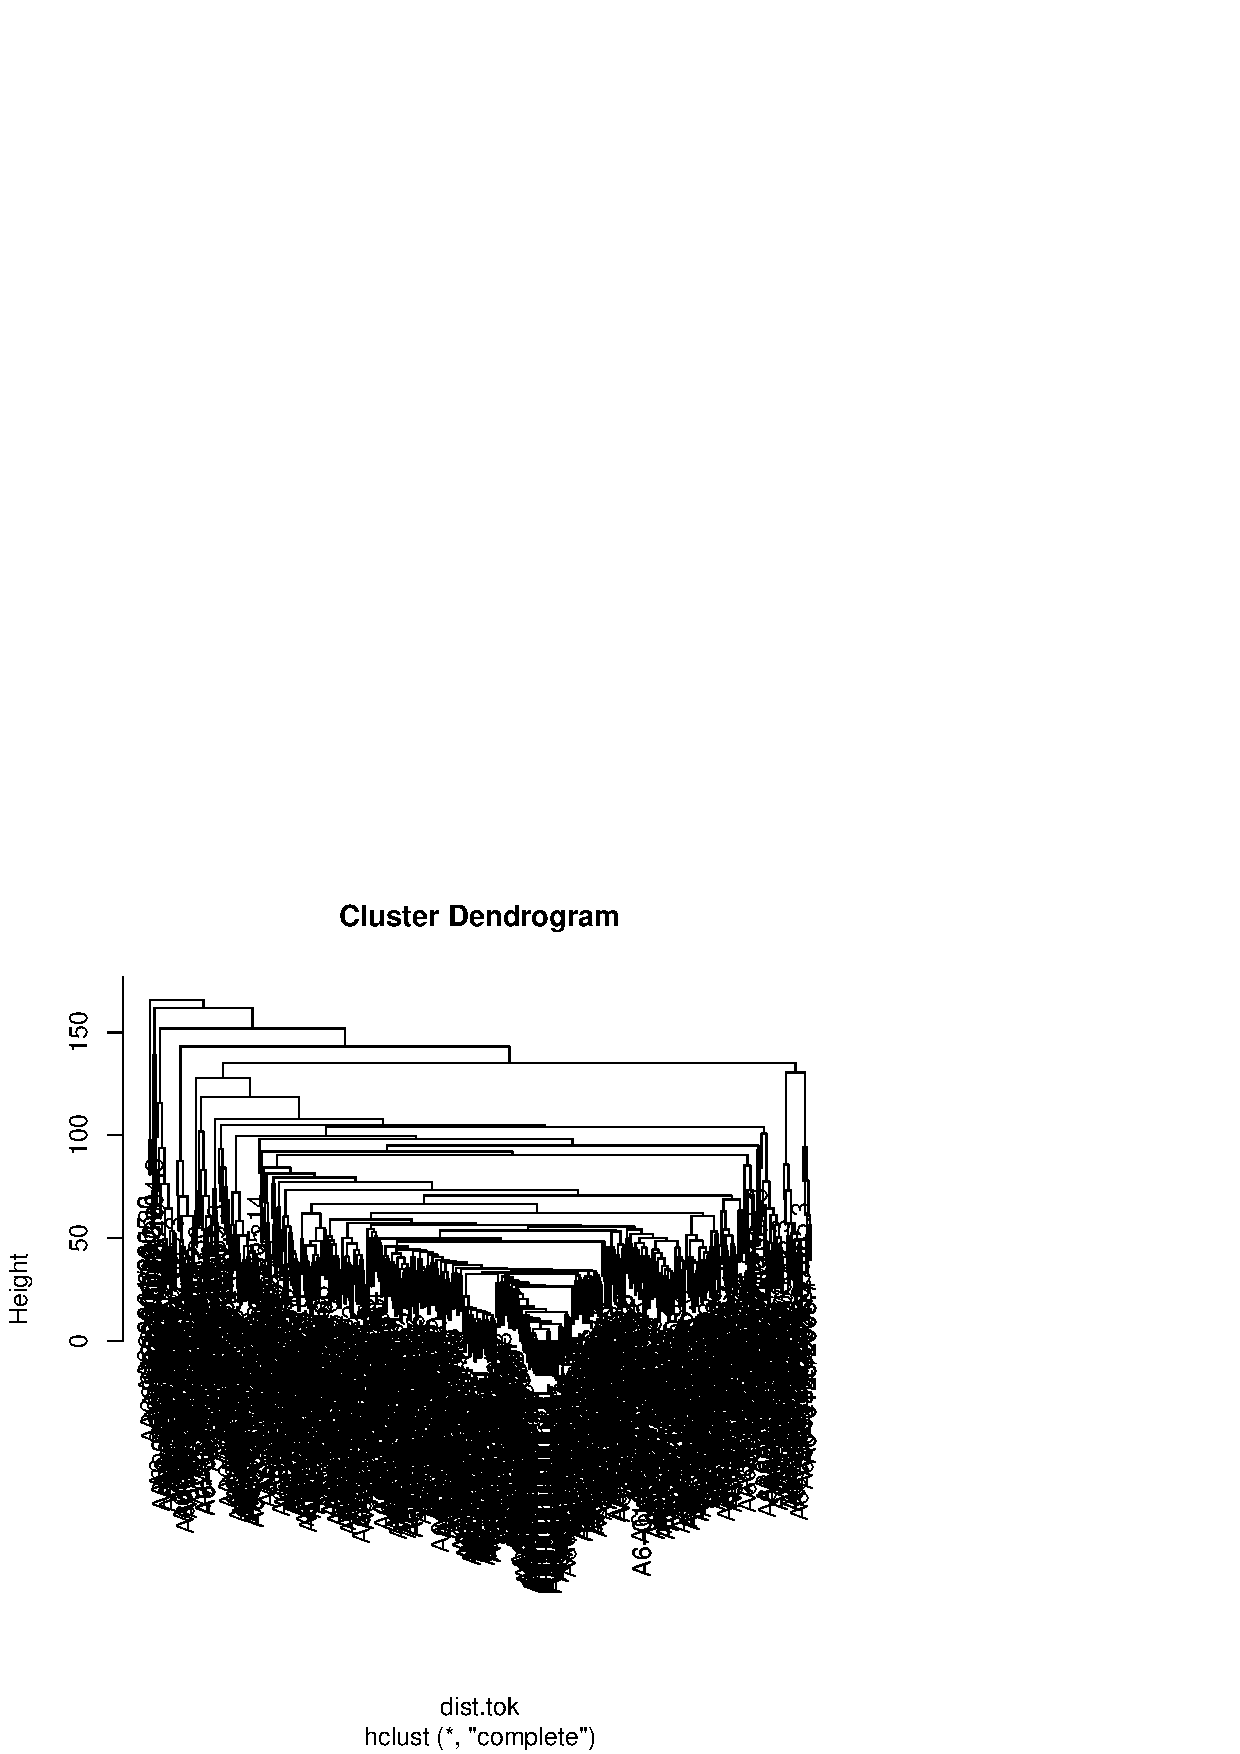
\includegraphics{intro-021}

In the preceding chunk of code we use \RSNL's \code{documentTokenMarix()}
method to extract an matrix of weighted---using the
\code{weightTfIdf} method provided by \tm---document-word frequencies
(rows are documents while columns represent tokens) and invoke the
\code{dist()} function in the \stats\ package to generate a distance
matrix suitable for hierarchical clustering methods.
\code{documentTokenMatrix()} returns a \rclass{DocumentTermMatrix} object
as defined by the \tm\ package.

\subsubsection{Document Filters}

The graph we just generated is, for lack of a better word, ugly.  But
we can take advantage of the hierarchical nature of the dataset, and
the meta-data encoded in our \rclass{RSNLCorpus} object, to generate a
more readable plot.  So far we've restricted our transforms and
filters to operations on individual tokens but we can also filter out
particular documents from a \rclass{CorpusView} using \RSNL's
\code{filterDocuments()} method.\footnote{See \tm's \code{tmFilter()}
method for an analogous function that directly modifies the corpus.}  For
example, the 475 speeches in our dataset come from a smaller set of
debates on particular pieces of legislation.  During the debate, the
rapporteur---the member of the European Parliament responsible for
guiding the legislation through parliament---almost always gives a
short informational speech describing the bill.  We can take advantage
of the meta-data attached to our corpus to identify the rapporteur
speeches in the dataset.  Furthermore, we can use this information to
generate a filtered view of the data and try our simple visualization
technique again, using only the rapporteurs' speeches, in hopes of
generating a representation of the data that can tell us something
about the similarity of the topics under debate.
\begin{Schunk}
\begin{Sinput}
> rap <- sapply(debates, meta, tag="ISRAPPORTEUR")
> debates.rap <- filterDocuments(debates.tok,
+   FunctionalDocumentFilter(function(x) rap == 1))
> dist.rap <- dist(documentTokenMatrix(debates.rap, weightTfIdf))
> clust.rap <- hclust(dist.rap)
> plot(clust.rap)
\end{Sinput}
\end{Schunk}
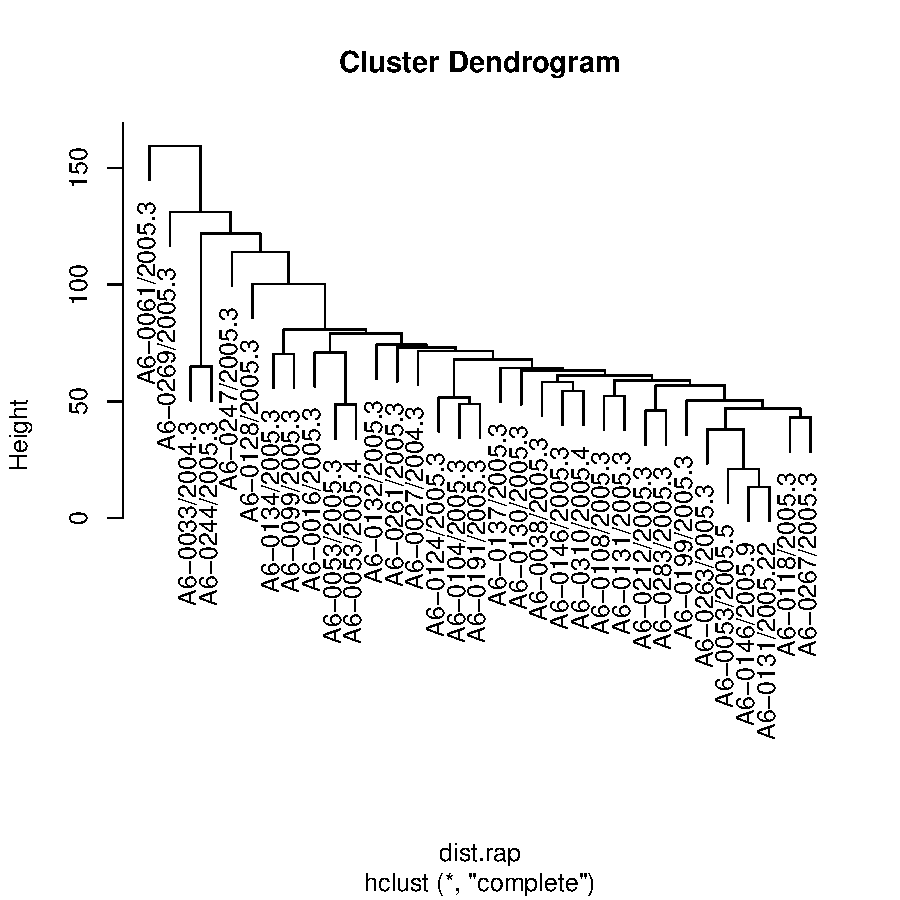
\includegraphics{intro-022}

Additionally, we might also try visualizing the rapporteur's speeches
from a bigram-based perspective:
\begin{Schunk}
\begin{Sinput}
> debates.rap.bigram <- filterDocuments(debates.bigram,
+   FunctionalDocumentFilter(function(x) rap == 1))
> dist.rap.bigram <- dist(documentTokenMatrix(debates.rap.bigram, weightTfIdf))
> clust.rap.bigram <- hclust(dist.rap.bigram)
> plot(clust.rap.bigram)
\end{Sinput}
\end{Schunk}
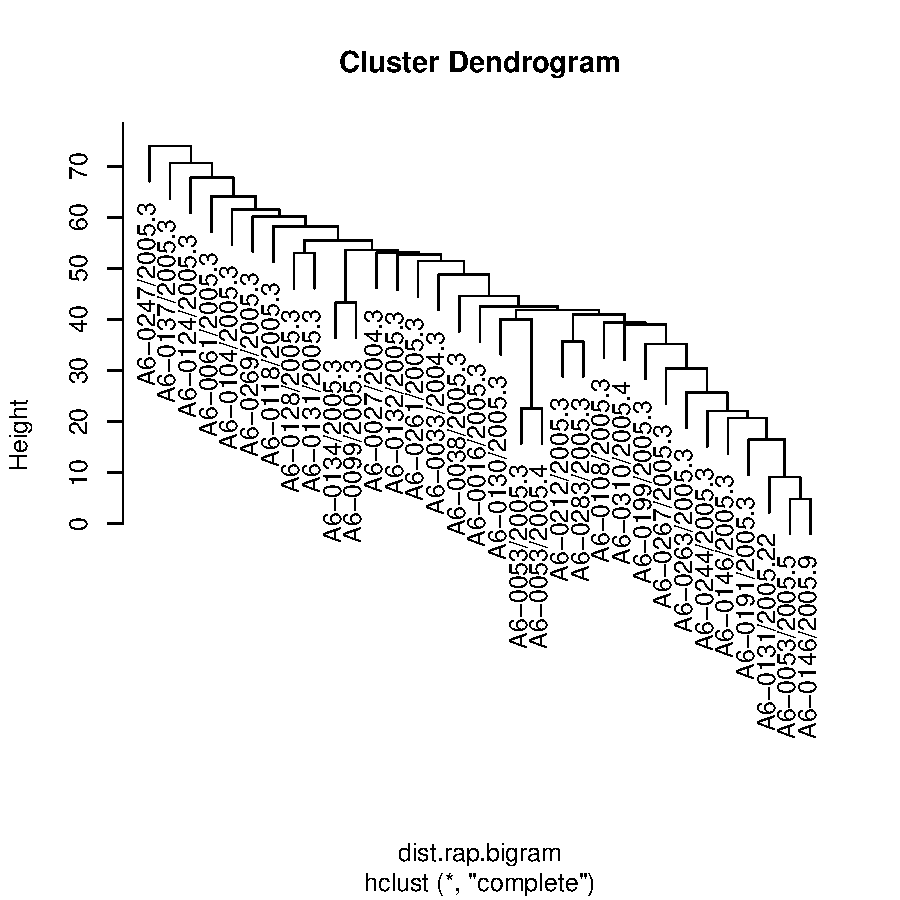
\includegraphics{intro-023}

\subsection{Tagging and Tagged Views}

So far we have dealt with simple tokenized representations of
documents and corpora.  \RSNL\ also provides tools for annotating
tokenized text with labels, or tags.  Tags provide information about
individual tokens in a view; one can use tags to annotate tokens with
part-of-speech information, entity type (e.g. person, place, or
thing), or any other piece of information the user might have about
individual tokens.  Tags allow users to incorporate semantic
information into their analyses and otherwise enhance the raw text
with pertinent token-level metadata.  In this section we demonstrate
how \RSNL\ represents text collections in terms of sequences of tagged
tokens, using \rclass{TaggedView} objects.  The \rclass{TaggedView}
types extend the \rclass{TokenizedView} classes; thus a
\rclass{TaggedCorpusView} is a type of \rclass{TokenizedCorpusView}
and a \rclass{TaggedDocumentView} is a sort
of\rclass{TokenizedCorpusView}.  Therefore, the methods we provide to
interrogate tokenized views---such as \code{documentTokenMatrix()},
\code{freq()}, \code{freqTable()}, \code{has()}, and
\code{unique()}---all operate on tagged views, although the output of
these methods may differ across types.  Furthermore, tagged views
provide a number of new methods that allow the user to effectively
take advantage of the token label information represented by these
views.

Because taggers often take advantage of case to do their work, we'll
copy over our all lowercase \code{debates} object before proceeding.
\begin{Schunk}
\begin{Sinput}
> debates <- RSNLCorpus(tm.debates)
\end{Sinput}
\end{Schunk}

\subsubsection{Applying a Tagger}

Tagging is similar to tokenization in practice and \RSNL\ provides a
method, \code{tag()} that can generate tagged tokens from a variety of
data types.  Tags are applied to tokens and \RSNL's taggers are
designed to apply tags to objects representing token vectors.
Given a \rclass{character} object, \code{tag()} will treat the object
as a vector of tags if it contains more than one element; on the other
hand, if the input contains only one element (or is a
\rclass{TextDocument} object), \code{tag()} will treat the input as
raw text and apply a tokenizer to it before tagging:
\begin{Schunk}
\begin{Sinput}
> tag(debates[[1]]) # Uses the default MaxentTagger and PTBTokenizer
\end{Sinput}
\begin{Soutput}
 [1] "The/DT"           "next/JJ"         
 [3] "item/NN"          "is/VBZ"          
 [5] "the/DT"           "report/NN"       
 [7] "-LRB-/-LRB-"      "A6-0027/NNP"     
 [9] "\\//VBD"          "2004/CD"         
[11] "-RRB-/-RRB-"      "by/IN"           
[13] "Mrs/NNP"          "Corbey/NNP"      
[15] "on/IN"            "the/DT"          
[17] "draft/NN"         "European/JJ"     
[19] "Parliament/NNP"   "and/CC"          
[21] "Council/NNP"      "Directive/NNP"   
[23] "amending/VBG"     "Directive/NNP"   
[25] "94\\/62\\/EC/NNP" "on/IN"           
[27] "packaging/NN"     "and/CC"          
[29] "packaging/VBG"    "waste/NN"        
[31] "./."             
\end{Soutput}
\begin{Sinput}
> tag(c("George Washington lived at Mount Vernon."), 
+     tokenizer=RegexTokenizer("\\s+", FALSE))
\end{Sinput}
\begin{Soutput}
[1] "George/NNP"     "Washington/NNP" "lived/VBD"     
[4] "at/IN"          "Mount/NNP"      "Vernon./NNP"   
\end{Soutput}
\begin{Sinput}
> tag(c("George Washington lived at Mount Vernon."), MaxentTagger("english"))
\end{Sinput}
\begin{Soutput}
[1] "George/NNP"     "Washington/NNP" "lived/VBD"     
[4] "at/IN"          "Mount/NNP"      "Vernon/NNP"    
[7] "./."           
\end{Soutput}
\begin{Sinput}
> tag(c("George", "Washington", "lived", "at", "Mount", "Vernon", "."),
+       NamedEntityTagger())
\end{Sinput}
\begin{Soutput}
[1] "George/PERSON"     "Washington/PERSON"
[3] "lived/O"           "at/O"             
[5] "Mount/LOCATION"    "Vernon/LOCATION"  
[7] "./O"              
\end{Soutput}
\end{Schunk}
The preceding code segment demonstrates the two types of taggers that
currently ship with \RSNL.  The first is a Maximum Entropy based
part-of-speech (POS) tagger developed by the Stanford Natural Language
Processing Group, providing pre-trained models for Arabic, Chinese,
English, and German text \cite{pos}.  The English tagger uses tag
codes from the Penn Treebank.  The appendix to this document contains
a list of tags and corresponding parts of speech; Penn's tagging
conventions are described in detail in the Treebank's part-of-speech
tagging guide \cite{ptb}.

\rclass{MaxentTagger}s are designed to operate on text that is
tokenized according to Penn Treebank conventions and thus should
generally always be fed token vectors and views generated with a
\rclass{PTBTokenizer}.  Nonetheless, it is possible to specify a
custom tokenizer when invoking \code{tag()}, as the second line of the
above example shows.  The second type of tagger is a Named Entity
Recognizer (NER), also developed by the Stanford NLP Group \cite{ner},
which assigns PERSON, LOCATION, and ORGANIZATION labels to English
text.

When applied to a \code{character} vector \code{tag()} returns a
vector of type \rclass{Tagged}.  \rclass{Tagged} is a simple extension
of the base \code{character} type that associates tags with tokens.
When printed to the screen \rclass{Tagged} elements are displayed in
token/tag format, but, internally, operations on \rclass{Tagged}
objects only see tokens unless they request tags explicitly.  One can
extract tags with \code{label()} and convert a \rclass{Tagged} object
to a \code{character} vector of the form token/tag with the
\code{flatten()} method:
\begin{Schunk}
\begin{Sinput}
> (tagged <- tag(c("George Washington lived at Mount Vernon.")))
\end{Sinput}
\begin{Soutput}
[1] "George/NNP"     "Washington/NNP" "lived/VBD"     
[4] "at/IN"          "Mount/NNP"      "Vernon/NNP"    
[7] "./."           
\end{Soutput}
\begin{Sinput}
> label(tagged)
\end{Sinput}
\begin{Soutput}
[1] "NNP" "NNP" "VBD" "IN"  "NNP" "NNP" "."  
\end{Soutput}
\begin{Sinput}
> flatten(tagged)
\end{Sinput}
\begin{Soutput}
[1] "George/NNP"     "Washington/NNP" "lived/VBD"     
[4] "at/IN"          "Mount/NNP"      "Vernon/NNP"    
[7] "./."           
\end{Soutput}
\end{Schunk}
Of course, one can also tag a \rclass{RSNLCorpus}, yielding a
view of the corpus, or generate a tagged view of a single document:
\begin{Schunk}
\begin{Sinput}
> (debates.pos <- tag(debates))
\end{Sinput}
\begin{Soutput}
A tagged corpus view with 179959 total tagged tokens,
 10489 unique tagged tokens, 9265 unique tokens, and 43 unique tags
\end{Soutput}
\begin{Sinput}
> (debates.pos.1 <- tag(debates, index=1))
\end{Sinput}
\begin{Soutput}
A tagged document view of A6-0027/2004.1 with 31 total tagged tokens,
 27 unique tagged tokens, 26 unique tokens, and 13 unique tags
\end{Soutput}
\end{Schunk}
It is also possible to generate a tagged view from a tokenized view,
inheriting the view's transforms and filters\footnote{As long as they
are tag-safe.  See Section~\ref{sec:tagtrans} for details.} in the process:
\begin{Schunk}
\begin{Sinput}
> debates.tok <- stem(tokenize(debates))
> tag(debates.tok)
\end{Sinput}
\begin{Soutput}
A tagged corpus view with 179959 total tagged tokens,
 10220 unique tagged tokens, 6194 unique tokens, and 43 unique tags
\end{Soutput}
\end{Schunk}

\subsubsection{Working with Tagged Views}

As with \rclass{TokenizedView} object, we can examine out
\rclass{TaggedView}s with a variety of methods.  First of all, we can
examine the tokens in a document just as we would in a standard
\rclass{TokenizedView}, except now the method returns an object of
type \rclass{Tagged}:
\begin{Schunk}
\begin{Sinput}
> tokens(debates.pos[[1]])
\end{Sinput}
\begin{Soutput}
 [1] "The/DT"           "next/JJ"         
 [3] "item/NN"          "is/VBZ"          
 [5] "the/DT"           "report/NN"       
 [7] "-LRB-/-LRB-"      "A6-0027/NNP"     
 [9] "\\//VBD"          "2004/CD"         
[11] "-RRB-/-RRB-"      "by/IN"           
[13] "Mrs/NNP"          "Corbey/NNP"      
[15] "on/IN"            "the/DT"          
[17] "draft/NN"         "European/JJ"     
[19] "Parliament/NNP"   "and/CC"          
[21] "Council/NNP"      "Directive/NNP"   
[23] "amending/VBG"     "Directive/NNP"   
[25] "94\\/62\\/EC/NNP" "on/IN"           
[27] "packaging/NN"     "and/CC"          
[29] "packaging/VBG"    "waste/NN"        
[31] "./."             
\end{Soutput}
\begin{Sinput}
> tokens(debates.pos.1)
\end{Sinput}
\begin{Soutput}
 [1] "The/DT"           "next/JJ"         
 [3] "item/NN"          "is/VBZ"          
 [5] "the/DT"           "report/NN"       
 [7] "-LRB-/-LRB-"      "A6-0027/NNP"     
 [9] "\\//VBD"          "2004/CD"         
[11] "-RRB-/-RRB-"      "by/IN"           
[13] "Mrs/NNP"          "Corbey/NNP"      
[15] "on/IN"            "the/DT"          
[17] "draft/NN"         "European/JJ"     
[19] "Parliament/NNP"   "and/CC"          
[21] "Council/NNP"      "Directive/NNP"   
[23] "amending/VBG"     "Directive/NNP"   
[25] "94\\/62\\/EC/NNP" "on/IN"           
[27] "packaging/NN"     "and/CC"          
[29] "packaging/VBG"    "waste/NN"        
[31] "./."             
\end{Soutput}
\end{Schunk}
We can also take a look at the most common words in the corpus,
although \code{freqTable()} now returns tagged-token frequencies by
default.  Nonetheless, we can use the optional \code{what} argument to
see both tag and token frequencies:
\begin{Schunk}
\begin{Sinput}
> sort(freqTable(debates.pos), dec=T)[1:20]
\end{Sinput}
\begin{Soutput}
 the/DT     ,/,     ./.   of/IN   to/TO  and/CC 
  10727    9467    6253    5710    5489    4823 
  in/IN  is/VBZ    a/DT  for/IN that/IN   I/PRP 
   3255    2832    2752    2383    2254    1871 
  on/IN   be/VB this/DT  we/PRP  it/PRP are/VBP 
   1658    1603    1573    1374    1195    1188 
 not/RB will/MD 
   1157     988 
\end{Soutput}
\begin{Sinput}
> sort(freqTable(debates.pos, what="Tokens"), dec=T)[1:20]
\end{Sinput}
\begin{Soutput}
  the     ,     .    of    to   and    in  that    is 
10727  9467  6253  5710  5489  4823  3261  3045  2832 
    a   for     I    on    be  this    we    it   are 
 2752  2383  1871  1665  1603  1573  1374  1195  1188 
  not  have 
 1157  1121 
\end{Soutput}
\begin{Sinput}
> sort(freqTable(debates.pos, what="Tags"), dec=T)[1:20]
\end{Sinput}
\begin{Soutput}
   NN    IN    DT    JJ   NNS     ,   NNP    VB    RB 
23689 22584 19178 12589 10248  9467  8757  7809  7804 
  PRP     .    CC    TO   VBZ   VBP   VBN    MD   VBG 
 6860  6386  5756  5515  4934  4458  4408  3501  2854 
   CD  PRP$ 
 2607  1701 
\end{Soutput}
\end{Schunk}
Similarly, we can generate lists of unique tagged tokens, tokens, and
tags
\begin{Schunk}
\begin{Sinput}
> u.tagtok <- unique(debates.pos)
> u.tok <- unique(debates.pos, what="Tokens")
> (u.tag <- unique(debates.pos, what="Tags"))
\end{Sinput}
\begin{Soutput}
 [1] "DT"    "JJ"    "NN"    "VBZ"   "-LRB-" "NNP"  
 [7] "VBD"   "CD"    "-RRB-" "IN"    "CC"    "VBG"  
[13] "."     ","     "NNS"   "VBN"   "NNPS"  "TO"   
[19] ":"     "PRP$"  "VB"    "RB"    "MD"    "JJR"  
[25] "RBR"   "RP"    "PRP"   "VBP"   "WDT"   "WRB"  
[31] "JJS"   "POS"   "RBS"   "EX"    "WP"    "PDT"  
[37] "``"    "''"    "WP$"   "FW"    "UH"    "LS"   
[43] "SYM"  
\end{Soutput}
\end{Schunk}
or generate document-token/tag/tagged-token matrices:
\begin{Schunk}
\begin{Sinput}
> documentTokenMatrix(debates.pos)
\end{Sinput}
\begin{Soutput}
A document-term matrix (475 documents, 9265 terms)

Non-/sparse entries: 86652/4314223
Sparsity           : 98%
Maximal term length: 26 
Weighting          : term frequency (tf)
\end{Soutput}
\begin{Sinput}
> documentTagMatrix(debates.pos)
\end{Sinput}
\begin{Soutput}
A document-term matrix (475 documents, 43 terms)

Non-/sparse entries: 12493/7932
Sparsity           : 39%
Maximal term length: 5 
Weighting          : term frequency (tf)
\end{Soutput}
\begin{Sinput}
> documentTaggedTokenMatrix(debates.pos)
\end{Sinput}
\begin{Soutput}
A document-term matrix (475 documents, 10489 terms)

Non-/sparse entries: 88542/4893733
Sparsity           : 98%
Maximal term length: 29 
Weighting          : term frequency (tf)
\end{Soutput}
\end{Schunk}

% THIS EXAMPLE IS NEAT BUT VERY RANDOM
%The methods available for working with tagged views provide the user
%with a rich array of tools with which to examine a corpus, and make it
%possible to perform surprisingly sophisticated operations in just a
%few lines of code.  For example, the following code snippet finds
%every word in the corpus that is used as both a singular noun and a
%verb in its base form and displays their frequencies:
%<<tag.coolexample>>=
%nv <- u.tok[sapply(u.tok, 
%  function (u)
%    has(debates.pos, Tagged(u, "NN")) & has(debates.pos, Tagged(u, "VB")))]
%
%sapply(nv,
%  function (token) sapply(c("NN", "VB"), 
%    function (tag) freq(debates.pos, Tagged(token, tag))))
%@

\subsubsection{Transforming and Filtering Tagged Views}\label{sec:tagtrans}

One can apply transforms and filters to tagged views, just as one may
with tokenized views.  Indeed, because a tagged view is a type of
tokenized view, one can apply a large variety of of token transforms
and filters directly to tagged views.  For example, we can remove
stopwords from a tagged view just as we might from a tokenized view:
\begin{Schunk}
\begin{Sinput}
> (debates.pos <- filterTokens(debates.pos, StopFilter()))
\end{Sinput}
\begin{Soutput}
A tagged corpus view with 83312 total tagged tokens,
 9743 unique tagged tokens, 8696 unique tokens, and 33 unique tags
\end{Soutput}
\end{Schunk}
Furthermore, when one generates a tagged view from a tokenized view,
the tagged view inherits the former's transforms:
\begin{Schunk}
\begin{Sinput}
> debates.tok <- tokenize(debates)
> debates.tok <- transformTokens(debates.tok, 
+   RegexTokenTransform("^[0-9]+$", "NUMBER"))
> debates.tok <- filterDocuments(debates.tok, # 20% sample
+   FunctionalDocumentFilter(function(x) runif(length(x)) < .8))
> (debates.pos <- tag(debates.tok))
\end{Sinput}
\begin{Soutput}
A tagged corpus view with 139138 total tagged tokens,
 9096 unique tagged tokens, 8052 unique tokens, and 42 unique tags
\end{Soutput}
\end{Schunk}
\RSNL\ also provides tools that make tag-based filtering especially
convenient.  For example, we can restrict a view to noun forms as follows:
\begin{Schunk}
\begin{Sinput}
> filterTokens(debates.pos, RegexTagFilter("^NN"))
\end{Sinput}
\begin{Soutput}
A tagged corpus view with 33776 total tagged tokens,
 4102 unique tagged tokens, 4035 unique tokens, and 4 unique tags
\end{Soutput}
\end{Schunk}
Along a similar vein, we can use the NER tagger to extend our cluster
analysis from the previous section.  This time we'll cluster debates
purely in terms of organizations mentioned, collapsing word counts
across speeches in the same debate:
\begin{Schunk}
\begin{Sinput}
> # Tag and filter
> debates.ner <- tag(debates, NamedEntityTagger())
> debates.ner <- filterTokens(debates.ner,
+   FunctionalTagFilter(function (x) x == "ORGANIZATION"))
> # Create a debate-token matrix
> docTM <- as.matrix(documentTokenMatrix(debates.ner))
> codes <- sapply(debates, meta, tag="CODE")
> ucodes <- unique(codes)
> debateTM <- t(sapply(ucodes, 
+   function (ucode) apply(docTM[codes==ucode, ], 2, sum)))
> # Calculate distances and plot
> dist.ner <- dist(debateTM)
> clust.ner <- hclust(dist.ner)
> plot(clust.ner)
\end{Sinput}
\end{Schunk}
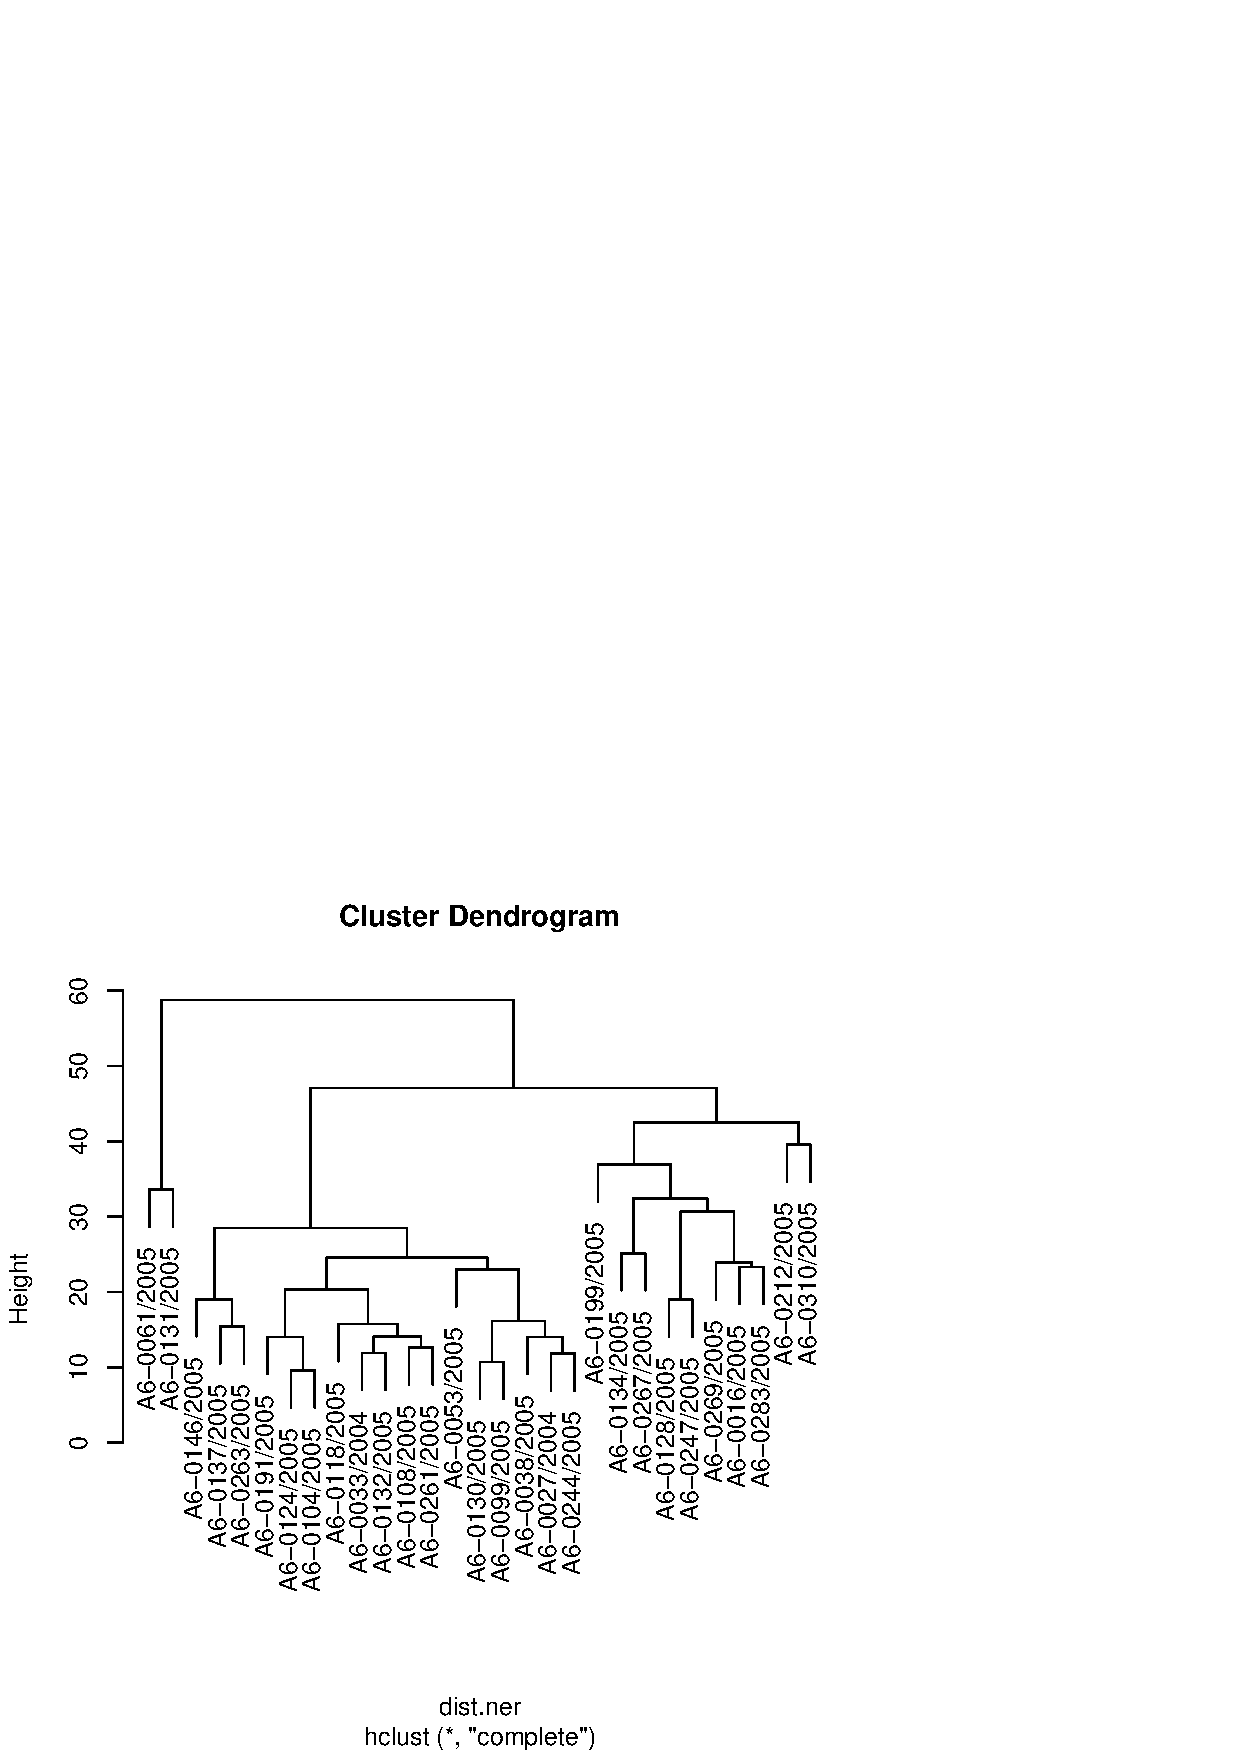
\includegraphics{intro-036}


It is important to realize that one does face some limitations when
applying token transforms to tagged views.  First of all, it is
important to note that \RSNL\ tokenizes and tags text prior to
applying token filters and transforms when constructing tagged views.
This is generally the behavior that the user wants---both the POS and
NER taggers are designed to operate on raw text and may perform poorly
on transformed, and especially filtered, input---but it is important
to keep in mind that transforms and filters are post-tag operations,
even for tagged views that are constructed from filtered and
transformed tokenized views.  Furthermore, while all document and
token filters are safe for use with tagged views the same does not
hold true for token transforms more generally.  The
\rclass{TokenTransform} interface requires only that a transform
provide a specialization of the \code{transformTokens} method that
takes a \code{character} vector as its first argument and returns a
transformed \code{character} vector.  Therefore, arbitrary transforms
may discard tag information when dealing with the contents of tagged
views.  To be tag-safe a transform must return an object of type
\rclass{Tagged} when a \rclass{Tagged} vector is passed as the first
argument to \code{transformTokens}.  For example, we can build a
tag-safe transform for converting tokens to upper case like so:
\begin{Schunk}
\begin{Sinput}
> ucTransform <- FunctionalTokenTransform(
+   function (x)
+     if (is(x, "Tagged"))
+       Tagged(toupper(x), label(x))
+     else
+       toupper(x), tagSafe=TRUE)
> sort(freqTable(transformTokens(debates.pos, ucTransform)), dec=T)[1:20]
\end{Sinput}
\begin{Soutput}
   THE/DT       ,/,       ./.     OF/IN     TO/TO 
     9479      7663      5119      4725      4482 
   AND/CC     IN/IN    IS/VBZ      A/DT    FOR/IN 
     3988      2957      2324      2284      1988 
  THAT/IN   THIS/DT     I/PRP    WE/PRP     ON/IN 
     1880      1560      1538      1487      1395 
NUMBER/CD    IT/PRP     BE/VB   ARE/VBP    NOT/RB 
     1340      1327      1312      1005       938 
\end{Soutput}
\end{Schunk}
Note that we indicate that \code{ucTransform} is a tag-safe object by
passing the argument \code{tagSafe=TRUE} to the
\rclass{FunctionalTokenTransform} constructor.  This causes the
constructor to generate a type of \rclass{FunctionalTokenTransform}
object that extends the \rclass{TagSafe} class, indicating that it
provides a tag-safe interface.\footnote{Note that passing
\code{tagSafe=TRUE} to the constructor does not guarantee tag-safety,
but rather provides an indicator that the transform conforms to the
\rclass{TagSafe} interface; that is, that it provides a specialization
of \code{transformTokens} that returns an object of type \code{Tagged}
when a \code{Tagged} vector is provided as its first argument.  Other
code may test transforms for tag-safety prior to applying them by
seeing if they extend the \rclass{TagSafe} class.}
Furthermore,  most of \RSNL's pre-built transform types---including
\rclass{RegexTokenTransform}, \rclass{SnowballStemmer}, and
\rclass{TolowerTokenTransform}---are tag-safe and implement the
\rclass{TagSafe} interface.

\section{Appendix: Penn Treebank Part of Speech Codes}

\begin{tabular}{ll}
CC & Coordinating conjunction \\
CD & Cardinal number \\
DT & Determiner \\
EX & Existential there \\
FW & Foreign word \\
IN & Preposition or subordinating conjunction \\
JJ & Adjective \\
JJR & Adjective, comparative \\
JJS & Adjective, superlative \\
LS & List item marker \\
MD & Modal \\
NN & Noun, singular or mass \\
NNS & Noun, plural \\
NNP & Proper noun, singular \\
NNPS & Proper noun, plural \\
PDT & Predeterminer \\
POS & Possessive ending \\
PRP & Personal pronoun \\
PRP\$ & Possessive pronoun \\
RB & Adverb \\
RBR & Adverb, comparative \\
RBS & Adverb, superlative \\
RP & Particle \\
SYM & Symbol \\
TO & to \\
UH & Interjection \\
VB & Verb, base form \\
VBD & Verb, past tense \\
VBG & Verb, gerund or present participle \\
VBN & Verb, past participle \\
VBZ & Verb, 3rd person singular present \\
WDT & Wh-determiner \\
WP & Wh-pronoun \\
WP\$ & Possessive wh-pronoun \\
WRB & Wh-adverb
\end{tabular}

\begin{thebibliography}{9}
 
\bibitem{tm}
  Ingo Feinerer, Kurt Hornik, David Meyer.
  2008.
  ``Text Mining Infrastructure in R.''
  \emph{Journal of Statistical Software} 25 (5).

\bibitem{ner}
  Jenny Rose Finkel, Trond Grenager, and Christopher Manning.
  2005.
  ``Incorporating Non-local Information into Information Extraction
  Systems by Gibbs Sampling.'' 
  Proceedings of the 43nd Annual Meeting of the Association for 
  Computational Linguistics (ACL 2005), pp.  363-370.
  http://nlp.stanford.edu/~manning/papers/gibbscrf3.pdf

\bibitem{rcv}
  Daniel Pemstein.
  2009.
  ``Predicting Roll Calls with Legislative Text.''
  Presented at \emph{The 67th Annual National Conference of the
  Midwest Political Science Association}.

\bibitem{ptb}
  Beatrice Santorini.  1990. ``Part-of-Speech Tagging Guidelines for the
  Penn Treebank Project (3rd Revision, 2nd Printing)''
  \url{ftp://ftp.cis.upenn.edu/pub/treebank/doc/tagguide.ps.gz}.

\bibitem{xml}
  Duncan Temple Lang.
  2008.
  ``XML: Tools for parsing and generating XML within R and S-Plus.''
  \url{http://cran.r-project.org/web/packages/XML/index.html}.

\bibitem{pos}
  Kristina Toutanova and Christopher D. Manning. 
  2000. 
  ``Enriching the
  Knowledge Sources Used in a Maximum Entropy Part-of-Speech
  Tagger.''  
  In Proceedings of the Joint SIGDAT Conference on Empirical
  Methods in Natural Language Processing and Very Large Corpora
  (EMNLP/VLC-2000), pp. 63-70.
 
\end{thebibliography}


\end{document}
